
%---------------------------------------------------------
\section{Introduction}
%---------------------------------------------------------

%---------------------------------------------------------
\subsection{History of running a software}
\begin{frame}
	\frametitle{History of running a software}
	\begin{itemize}
		\item Install or use an existing operating system.
		\item Install the tools used by your software.
		\item Install dependencies of your software.
		\item Run your software.
		\item Repeat or reuse for every new software version release.
	\end{itemize}
\end{frame}
%---------------------------------------------------------

%---------------------------------------------------------
\section{Virtualization}
%---------------------------------------------------------

%---------------------------------------------------------
\subsection{Virtual Machines}
\begin{frame}
	\frametitle{Virtual Machines}
	\begin{itemize}
		\item Virtual machines (VMs) are an abstraction of physical hardware, turning one server into many servers.
		\item The hypervisor allows multiple VMs to run on a single machine.
		\item Each VM includes a full copy of an operating system, the application, necessary binaries, and libraries - taking up tens of GBs.
		\item Virtual machines are
		\begin{itemize}
			\item portable,
			\item reproducable,
			\item controlled,
			\item and can be provided upon user reuest withing minutes.
		\end{itemize}
	\end{itemize}
\end{frame}
%---------------------------------------------------------

%---------------------------------------------------------
\subsection{Infrastructure as a service - IaaS}
\begin{frame}
	\frametitle{Infrastructure as a service - IaaS}
	Provisioning virual machines and providing them as a service among other services (ex. networking services) by a cloud operaor is IaaS.
	\newline
	\begin{itemize}
		\item Famous cloud IaaS providers
		\begin{itemize}
			\item AWS - EC2 [Elastic Compute Cloud].
			\item GCP - Compute Engine.
		\end{itemize}
	\end{itemize}
\end{frame}
%---------------------------------------------------------

%---------------------------------------------------------
\section{Containerization}
%---------------------------------------------------------

%---------------------------------------------------------
\subsection{Issues and motive behind containerization}
\begin{frame}
	\frametitle{Issues and motive behind containerization}
	\begin{itemize}
		\item VMs can be slow to boot.
		\item VMs are relatively big (compared to executed software)
		\item Containerization eliminates the quote, "it worked on my machine." (\textbf{Low risk of failing in production}).
		\item Containerization eliminates the installation and configuration time. (\textbf{Easy and fast deployment}).
		\item Containerization packages Software into Standardized Units for Development, Shipment, and Deployment. (\textbf{Isolation}).
		\item Containerization eliminates infrastructure wasted resources and utilizes them.
		\item Containerization easy the scalability dilemma.
	\end{itemize}
\end{frame}
%---------------------------------------------------------

%---------------------------------------------------------
\subsection{What is a Container?}
\begin{frame}
	\frametitle{What is a Container?}
	\begin{itemize}
		\item A container is an abstraction at the app layer that packages code and dependencies together as a standardized unit of software..
		\item Multiple containers can run on the same machine and share the OS kernel with other Containers, each running as isolated processes in userspace.
		\item Containers take up less space than VMs (container images are typically tens of MBs in size), can handle more applications, runs quickly and reliably.
		\item A container image is apersisted, lightweight, standalone, executable package of software that includes everything needed to run an application: code, runtime, system tools, system libraries, and settings.
	\end{itemize}
\end{frame}
%---------------------------------------------------------

%---------------------------------------------------------
\subsection{Containers VS Virtual Machines}
\begin{frame}
	\frametitle{Containers VS Virtual Machines}
	Containers and virtual machines have similar resource isolation and allocation benefits but Containers virtualize the operating system instead of the hardware.
	\linebreak
	
	\centering
	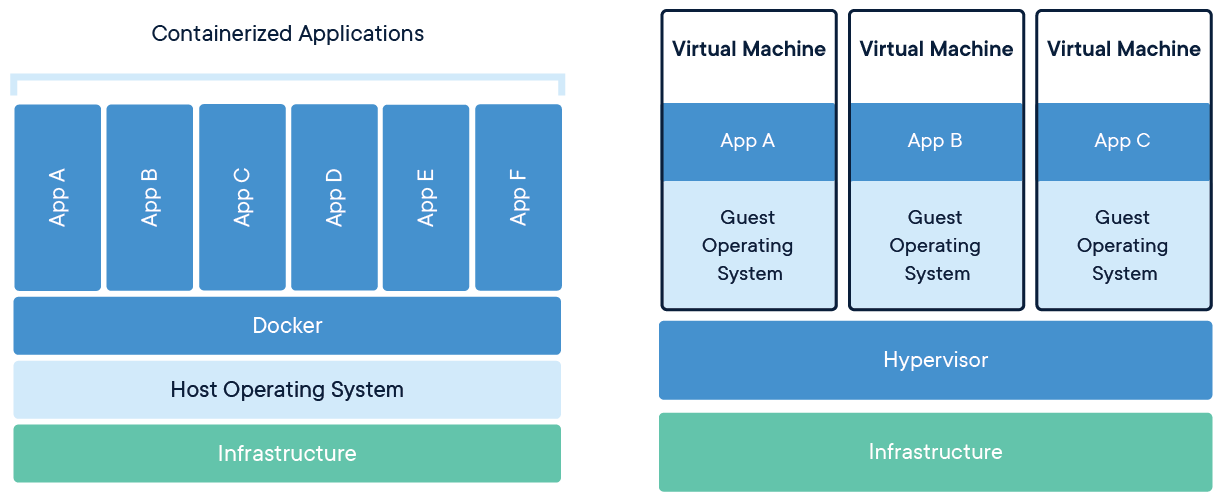
\includegraphics[width=\linewidth]{figures/docker-containerized-and-vm-transparent-bg.png}
\end{frame}
%---------------------------------------------------------

%---------------------------------------------------------
\subsection{Container-based virtualization Solutions}
\begin{frame}
	\frametitle{Container-based virtualization Solutions}
	\begin{itemize}
		\item \textbf{Docker} is the most popular, and we will explain briefly.
		\item \textbf{OpenVZ}
		\item \textbf{LXC} Linux containers 
	\end{itemize}
\end{frame}
%---------------------------------------------------------

%---------------------------------------------------------
\section{References}
\begin{frame}
	\frametitle{References}
	\begin{itemize}
		\item \href{https://www.docker.com/resources/what-container}{Docker - What is a container?}
		\item \href{https://openvz.org/}{OpenVZ}
		\item \href{https://linuxcontainers.org/}{Linux Containers}
	\end{itemize}
\end{frame}
%---------------------------------------------------------
